% vim: set spelllang=fr foldmethod=marker:

\lettrineh{L}{e \chapref{sa}} expose un algorithme de sélection pseudo-aléatoire des nœuds de surveillance.
L'un des inconvénients de cet algorithme est que l'énergie résiduelle des capteurs, \cad le niveau d'énergie restant dans leur batterie, n'est pas mesurée, et surtout n'est pas prise en compte lors du processus de renouvellement des \cns.
Pourtant, la surveillance que ces derniers mènent dans leur cluster entraine une consommation énergétique accrue, puisqu'ils doivent demeurer en écoute sur le médium de façon continue.

Dans ce chapitre, une deuxième méthode de sélection des \cns est introduite.
Le concept initial de l'algorithme est extrêmement simple: à chaque renouvellement du processus, l'énergie résiduelle des capteurs est évaluée, et ceux possédant le plus de réserves deviennent \cns.
Le but de cette méthode est évidemment d'atteindre une meilleure répartition de la consommation d'énergie dans le cluster: les capteurs possédant le plus haut niveau de charge de leur batterie se verront attribuer le rôle qui consomme le plus d'énergie.

Néanmoins, la perte de l'aspect aléatoire au profit d'une méthode purement déterministe va entrainer un certain nombre de contraintes en termes de sécurité et de couverture spatiale.
Il faut donc mettre en place des parades face aux nœuds compromis qui tenteraient de conserver \textit{ad~vitam~æternam} le rôle de \cn en falsifiant leur niveau d'énergie.
Un nouveau type de nœuds, les \vns, viennent ici prévenir les tentatives de fraudes, tandis que le \ch veille à la couverture correcte du réseau par les \cns.
Les performances obtenues à l'aide de ce second mécanisme de sélection sont elles aussi étudiées à travers un jeu de simulations.

\section{Mécanisme de sélection des \cns}\label{se:sec:proposal}

    \subsection{Utilisation des \vns pour sécuriser le processus de sélection}\label{se:subsubsec:elec1}

Les hypothèses présentées en début de \chapref{sa} (\ssref{sa:ssec:hypotheses}) demeurent valables ici.
Le processus de sélection dans ce chapitre repose sur l'énergie restante pour chaque nœud au moment du renouvellement.
Cette énergie disponible dans la batterie est dite «énergie résiduelle».
Afin de répartir au mieux la charge, les nœud possédant le plus d'énergie en réserve sont sélectionnés pour assurer la tâche qui consomme le plus.
Mais l'usage de la valeur d'énergie résiduelle comme critère de sélection présente un inconvénient notable: il n'y a aucun agent, dans le réseau, capable de mesurer de façon fiable le niveau d'énergie présent dans la batterie d'un nœud donné, si ce n'est ce nœud lui-même.
Les nœuds voisins d'un nœud $N$ peuvent tout au plus enregistrer les messages envoyés par $N$, et en inférer une valeur approximative de l'énergie consommée.
Mais ils ne connaissent ni le niveau d'énergie initial de $N$ (au moment du déploiement du réseau) ni l'énergie dépensée par $N$ lors de l'écoute du médium de transmission, la consommation approximative calculée ne permet pas de déduire le niveau d'énergie résiduelle avec une précision suffisante pour classer les nœuds de façon fiable sur ce critère.

Aussi la seule façon d'obtenir le niveau de charge de la batterie d'un nœud est-elle de le lui demander.
L'algorithme de sélection proposé s'écrit donc de la manière suivante:
\begin{enumerate}
    \item Au cours d'une première phase, chaque nœud évalue la valeur de son énergie résiduelle et la transmet au \ch;
    \item Une fois cette phase terminée (lorsque le \ch a reçu la valeur de chaque nœud, ou lorsque le délai d'attente a expiré), le \CH sélectionne les $n$ capteurs possédant le niveau d'énergie le plus élevé (où $n$ représente le nombre de \cns que l'on souhaite obtenir durant chaque cycle) et envoie à ceux-ci un message de notification pour leur assigner leur rôle de \cn.
\end{enumerate}
Cet algorithme est déterministe, et élimine tout aspect aléatoire du processus de sélection.
La règle est simple: les $n$ nœuds possédant le plus d'énergie en réserve au moment de la sélection sont désignés.
Comme le rôle de \cn est censé impliquer une consommation plus élevée en ressources énergétiques, la rotation des rôles est théoriquement assurée.

Mais l'aspect entièrement déterministe du processus peut aussi représenter une faille qui pourrait être exploitée par des nœuds compromis souhaitant s'assurer d'être sélectionnés.
Un attaquant a effectivement intérêt à faire attribuer le rôle de \cn aux nœuds qu'il a compromis, car cela lui permet:
\begin{itemize}
    \item de réduire le nombre de \cns légitimes dans le réseau capables de détecter les capteurs compromis;
    \item de signaler au \ch des capteurs «innocents» comme étant compromis, dans le but de les faire exclure du réseau.
\end{itemize}
Quand un algorithme de sélection (pseudo-)aléatoire est appliqué, un nœud compromis peut très bien être désigné pour un cycle, mais il perdra rapidement son rôle de surveillance, pour les cycles suivants.
Même avec un processus d'auto-désignation (basé sur le modèle de \leach par exemple), les nœuds compromis pourraient tenter de conserver leur rôle de \cn sur plusieurs cycles, mais cela n'empêcherait pas des capteurs légitimes de s'auto-désigner également.
Avec un processus déterministe, les nœuds compromis peuvent en revanche monopoliser la plupart des rôles de \cns.
Tout ce qu'ils ont à faire, pour en arriver là, consiste à annoncer un niveau de charge batterie plus élevé que celui des capteurs légitimes lors de la première phase de l'algorithme de sélection.
Ils sont alors assurés d'être désignés \cns; et s'il se trouve y avoir au moins $n$ nœuds compromis au sein du cluster, ils peuvent de cette manière accaparer les $n$ rôles de \cn et désactiver du même coup le mécanisme de détection dans son intégralité.
L'attaque devient alors impossible à détecter et à contrer.

Pour empêcher les capteurs de «mentir» lorsqu'ils annoncent leur valeur d'énergie résiduelle, l'assignation d'un nouveau rôle à certains des voisins de chaque \cn est proposée.
Ces nœuds, que nous appelleront désormais \vns (comme pour \textit{nœuds de vérification}), seront responsables de vérifier la consommation en énergie des nœuds de surveillance.
Une fois que la sélection des \cns est réalisée, chaque voisin d'un \cn nouvellement désigné choisit à partir d'un seuil de probabilité prédéfini s'il sera ou non \vn pour ce \cn.
Un capteur peut assumer le rôle de \vn pour plusieurs \cn différents, du moment qu'il s'agit de nœuds voisins.

Si le rôle de \vn s'avère trop gourmand en énergie, il devient inutile: autant déployer dès le départ, dans ce cas, un mécanisme de sélection pseudo-aléatoire des \cns.
Aussi les \vns ne doivent-ils pas demeurer en permanence à l'écoute du médium, comme le font les \cns.
Ils se contentent d'envoyer, de temps en temps, une requête au \cn qu'ils surveillent, pour lui demander son niveau d'énergie.
Ils conservent la réponse du \cn en mémoire.

Une fois qu'ils ont collecté suffisamment de données, les \vns essayent d'établir une corrélation entre le modèle théorique de la consommation du \cn surveillé, et les valeurs que celui-ci annonce (valeurs obtenues à la fois lors des phases de sélection et en réponse aux requêtes).
Quatre cas sont alors susceptibles de se produire:
\begin{enumerate}
    \item La consommation en énergie annoncée par le \cn ne correspond pas du tout au modèle théorique: il y a alors une forte probabilité pour que le nœud soit corrompu, et cherche à accaparer le rôle de \cn. Il est dénoncé au \ch;
    \item La consommation annoncée correspond très exactement au modèle théorique: le capteur est probablement un nœud compromis qui tente d'être sélectionné tout en échappant à la détection des \vns. Autrement dit: le nœud est compromis, mais il adapte son comportement par rapport au point précédent. Mais il est quasiment impossible en pratique que les valeurs théoriques et empiriques soient exactement identiques, sans la moindre marge d'erreur. Le capteur est donc dénoncé au \ch;
    \item La consommation correspond à peu près aux valeurs du modèle théorique, mais elle n'évolue pas dans le sens de la consommation réelle observée localement par les \vns (l'évolution locale dans le temps du \cn devrait être grossièrement similaire à celle des \vns, puisqu'ils sont voisins, mais ce n'est pas le cas). Il s'agit probablement d'un nœud compromis qui adapte son comportement par rapport aux deux premiers points, par exemple en décrémentant son énergie des montants minimum imposés par la marge d'erreur définie vis à vis du modèle théorique. Le nœud est dénoncé au \ch;
    \item La consommation annoncée correspond grossièrement au modèle théorique, et évolue dans le sens de la consommation locale observée par les \vns. Que le nœud soit compromis ou non, il adopte ici un comportement normal, et est autorisé à endosser le rôle de \cn.
\end{enumerate}
Si un \vn est compromis, il peut tenter de faire exclure le \cn légitime qu'il observe.
Le \ch doit donc recevoir les rapports de plusieurs \vns distincts (selon un seuil prédéterminé) avant de considérer un \cn comme étant réellement compromis.
Dans une certaine mesure, cette précaution permet aussi de protéger un \cn légitime des erreurs (faux positifs) de ses \vns.

Le recours au rôle de \vn assure ainsi que seuls les nœuds annonçant un niveau d'énergie résiduelle plausible seront autorisés à agir en temps que \cns.
Comme ce dernier rôle consomme plus d'énergie que le relevé et la transmission des mesures sur l'environnement des capteurs, les nœuds sélectionnés pour être \cns verront tôt ou tard leur énergie résiduelle descendre sous le niveau des nœuds assurant leurs fonctions de base; une fois ce stade atteint, ils sont assurés de perdre leur rôle pour le cycle suivant.
On remarquera que les points~2 et~3 énoncés ci-dessus correspondent à un nœud compromis qui décrémente volontairement son énergie annoncée au cours du temps; même si des irrégularités peuvent être détectées et le nœud compromis être ainsi démasqué, le seul fait qu'il applique ce comportement assure tout de même que le capteur compromis cessera d'être désigné \cn pour un cycle ou pour un autre dans le futur.

Le modèle énergétique implémenté par les \vns pour vérifier les affirmations des \cns ne doit pas être trop lourd, mais il doit demeurer suffisamment précis pour pouvoir déterminer si un \cn s'en éloigne véritablement, tout en limitant les faux positifs.
Nous proposons ici d'utiliser le modèle de diffusion de \textsc{Rakhmatov} et \textsc{Vrudhula}~\cite{RV01}.\label{se:rakvru-formula}
Ce choix repose sur plusieurs observations:
\begin{itemize}
    \item Ce modèle fournit une approximation assez précise de la consommation réelle d'une batterie, et tient compte des processus chimiques internes à la batterie tels que les effets de récupération (\textit{recovery effect} en anglais) ou de perte de capacité selon la tension de décharge (\textit{rate capacity effect});
    \item Il s'agit de l'un des modèles implémentés dans \nsiii, ce qui permet, pour les simulations basées sur ce logiciel, de bénéficier d'une implémentation déjà existante, et surtout d'un modèle théorique parfait. Il ne faut pas craindre cependant que ce modèle ne soit «trop parfait» pour être utilisé par les \vns, étant donné que ces derniers estimeront l'énergie consommée par les \cns à partir de messages émis par ces derniers, sans connaissance des mécanismes internes au nœud (calcul, écoute) comme le fait le cœur du simulateur. Les valeurs calculées par les \vns demeurent donc approximatives par rapport à la consommation des \cns réellement calculée par \nsiii.
\end{itemize}
Le modèle de diffusion de \textsc{Rakhmatov} et \textsc{Vrudhula} se réfère aux réactions chimiques qui se produisent à l'intérieur de l'électrolyte de la batterie, et elle est résumée par l'\equaref{se:eqn:rvdm}
\begin{equation}
    \label{se:eqn:rvdm}
    \sigma(t) = \underbrace{\int_{0}^{t} i(\tau) \, \mathrm d\tau}_{l(t)} \;+\; \overbrace{\int_{0}^{t} i(\tau) \left(2 \sum_{m=1}^{\infty} \exp^{-\beta^2 m^2 (t-r)} \right) \mathrm d\tau}^{u(t)}
\end{equation}
où:
\begin{itemize}
    \item $\sigma(t)$ est la charge apparente perdue par la batterie à l'instant $t$;
    \item $l(t)$ est la charge «utile»;
    \item $u(t)$ est la charge inutilisable («perdue dans la batterie»);
    \item $i(t)$ est l'intensité du courant électrique à l'instant $t$;
    \item $\beta = \dfrac{\pi\sqrt{D}}{w}$, où $D$ est une constante de diffusion et $w$ la largeur de l'électrolyte.
\end{itemize}
En pratique, le calcul des dix premiers termes de la somme fournit une bonne approximation ---~il s'agit par ailleurs du comportement par défaut de \nsiii pour l'utilisation de ce modèle énergétique.

L'intérêt des \vns peut être résumé ainsi: un nœud compromis ne peut pas accaparer indéfiniment le rôle de \cn sans tricher lors des annonces, auquel cas ils sont détectés par les \vns.
La détection des \cns corrompus, ou bien le fait de les forcer à abandonner leur rôle pour un cycle futur, sont donc les deux objectifs des \vns.
Ce rôle n'empêche pas, par ailleurs, le nœud qui l'endosse de poursuivre ses activités de mesure: les requêtes auprès des \cns ne doivent pas survenir trop souvent, sous peine de décharger trop rapidement la batterie des \vns.
La machine à états des capteurs est présentée en \figref{se:fig:states}.
\begin{figure}[p]
    \centering
    \newlength\figuretotextheight
    \setlength\figuretotextheight\textheight
    \addtolength\figuretotextheight{-\abovecaptionskip}
    \addtolength\figuretotextheight{-\baselineskip}
    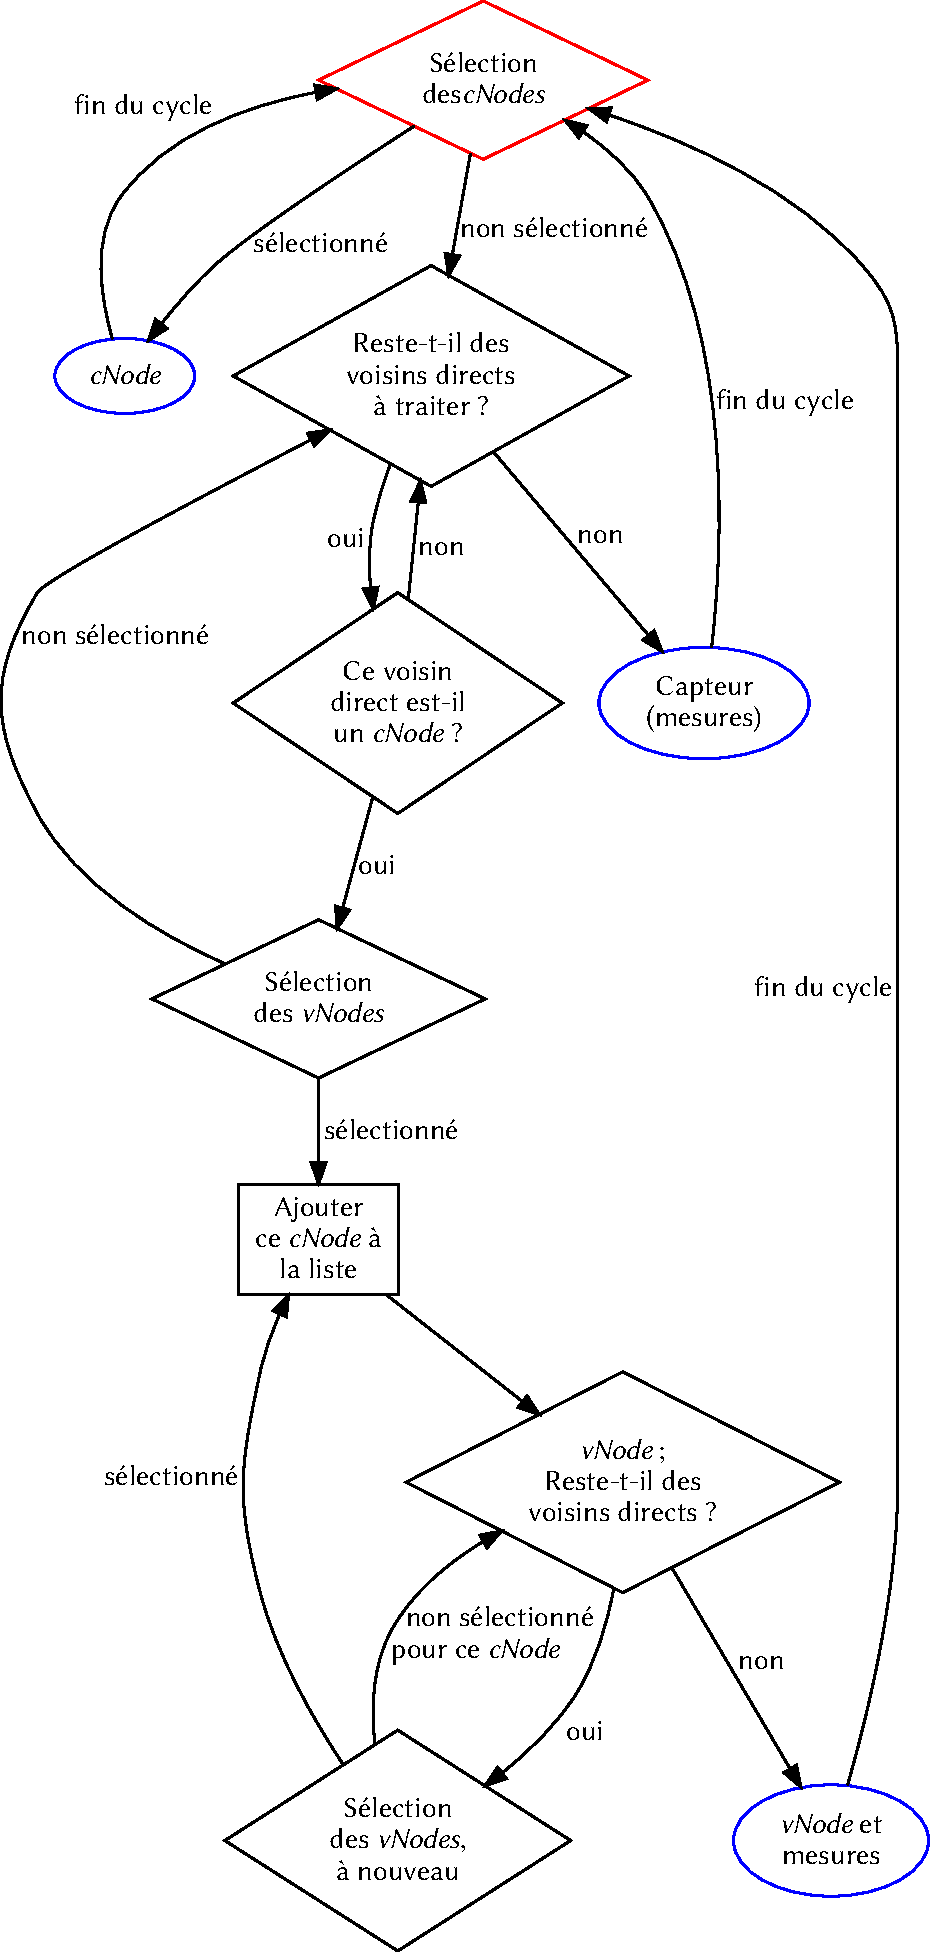
\includegraphics[height=\figuretotextheight]{\chapterfig/state_graph_vert.pdf}%
    \caption{Machine à états des capteurs (non-\cn)}\label{se:fig:states}%
\end{figure}

    \subsection{Couverture du cluster en cas d'activité hétérogène}

Le passage d'un algorithme pseudo-aléatoire à un processus de sélection déterministe n'a pas pour seul inconvénient d'introduire une faille que des capteurs compromis pourraient tenter d'exploiter.
Il soulève un second problème, indépendant du comportement des nœuds, qui pourrait gêner la détection de capteurs compromis.
S'il advient qu'une certaine zone géographique du cluster produit un trafic plus important que le reste des nœuds, alors l'énergie des capteurs de cette zone diminuera plus rapidement.
Il s'ensuit mécaniquement que les \cns ne seront pas ou peu sélectionnés parmi les capteurs de cette zone.
Il y a même de forte chances que les $n$ \cns désirés soient sélectionnés en dehors de la zone en question, et que certains capteurs ne soient pas surveillés du tout tant que le trafic de la zone d'activité ne diminue pas ---~potentiellement pour tous les cycles.
La figure \figref{se:fig:cover} illustre ce problème.
\begin{figure}[ht]
    \centering
    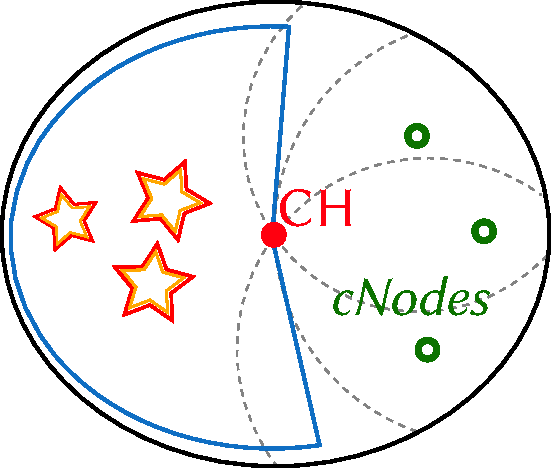
\includegraphics[width=.8\linewidth]{\chapterfig/cover.pdf}
    \caption{Schéma d'explication: les \cns sont sélectionnés au sein de la zone où l'activité est la plus faible (donc ou les nœuds ont conservé le plus d'énergie), et leur surveillance ne couvre pas les capteurs situés dans la partie opposée du cluster.}\label{se:fig:cover}
\end{figure}

Pour assurer une couverture complète du réseau, il est nécessaire de s'assurer que chaque capteur est surveillé par au moins un \cn.
Aussi l'algorithme de sélection présenté plus haut doit-il être modifié, pour devenir:
\begin{enumerate}
    \item Au cours d'une première phase, chaque nœud évalue la valeur de son énergie résiduelle et la transmet au \ch;
    \item Le \ch écoute toutes les valeurs. Les autres nœuds enregistrent également les valeurs de leurs voisins;
    \item Tous les nœuds envoient au \CH la liste de leurs voisins directs (\textit{1-hop})\,\footnote{Nous supposons ici que les capteurs ne trichent pas durant cette étape. Ils pourraient en effet annoncer des voisins «virtuels» supplémentaires, pour faire croire qu'ils seront à portée d'un \cn, et ainsi éviter d'être détecté si ce n'est pas le cas. Le \chapref{ea} présente des mécanismes de protection permettant de détecter ce type d'attaques.};
    \item Le \CH sélectionne les $n$ \cns parmi les nœuds ayant le plus d'énergie résiduelle, de telle façon que ces $n$ nœuds couvrent tous les autres nœuds en terme de portée\,\footnote{Les détails de l'algorithme utilisé pour cette phase ne sont pas précisés dans cette étude.};
    \item Au besoin (si $n$ est trop bas), le \CH sélectionne des \cns supplémentaires de façon à ce qu'ils couvrent l'intégralité du cluster;
    \item Le \CH envoie un message aux nœuds sélectionnés pour leur notifier leur rôle de \cn.
\end{enumerate}

Il est intéressant de noter que certains algorithmes de clusterisation (\heed~\cite{YF04} par exemple) utilisent d'autres mécanismes de sélection basés sur l'énergie résiduelle des nœuds ---~pour choisir des \chs, mais qui pourraient être transposer à la sélection des \cns.
Nous ne souhaitons pas utiliser dans ce chapitre de telles solutions qui n'utilisent l'énergie que comme l'un des paramètres pris en compte, et reposent donc sur la confiance vis à vis des nœuds qui calculent leur score propre.
Au contraire, nous préférons obtenir l'énergie annoncée par les nœuds pour la comparer au modèle théorique, et permettre ainsi aux \vns de veiller à la sécurité du processus.

    \subsection{Observations}

\paragraph{Mécanisme de détection}
La détection des attaques par \dds est inchangée par rapport au chapitre précédent.
Les \cns appliquent un ensemble de règles sur le trafic collecté dans le cluster: lorsqu'un capteur enfreint une règle un certain nombre de fois, par exemple lorsque le débit des paquets qu'il envoie excède un seuil prédéterminé, il est considéré comme malveillant (voir le paragraphe à ce sujet au \chapref{ea}, \ssref{ea:par:rules}).

\paragraph{Alourdissement du modèle}
La solution introduite de par le recours aux \vns consiste littéralement à choisir des nœuds chargés de surveiller les surveillants: le concept de surveillance devient récursif.
Le processus de sélection lui-même est alourdi par les messages des nœuds à destination de leur \ch, annonçant leur énergie résiduelle et la liste de leurs voisins.
Il est évident que la complexité de l'algorithme de sélection, et par suite logique celle de l'implémentation du système, s'en retrouvent rehaussées par rapport au mécanisme de sélection pseudo-aléatoire des \cns.

\paragraph{Allègement possible}
Les \vns sont utilisés pour empêcher les nœuds compromis de conserver un rôle de \cn sur plusieurs cycles sans être détectés.
Lors du premier cycle où un nœud donné occupe le rôle de \cn, il n'y a donc guère d'intérêt à le surveiller: il est statistiquement plus probable qu'il s'agisse d'un nœud légitime plutôt que compromis, et il a de bonnes chances d'abandonner le rôle au cycle suivant.
Le rôle de \vn pour un \cn donné peut donc attendre, pour être assigné, le deuxième cycle consécutif pendant lequel le \cn occupe son rôle.

\paragraph{Sécurité du réseau}
Il est intéressant de se pencher sur un autre point: l'usage des \cns combinés aux \vns n'apporte pas de garantie totale sur la sécurité du réseau.
Le système repose sur plusieurs hypothèses, comme le fait que des nœuds compromis ne collaborent pas ensemble: un capteur compromis sélectionné comme \cn pourrait annoncer au \ch, par exemple, qu'il peut entendre et surveiller une portion plus large du cluster que ce qu'il en est réellement, dans le but de faire croire au \CH que tout le cluster est surveillé~--- alors qu'en réalité ce ne sera pas le cas.
Si le \CH ne désigne aucun autre \cn pour surveiller ces zones, d'autres nœuds compromis pourraient y porter des attaques sans risque d'être détectés.
Une seconde hypothèse à prendre en compte établit que le \ch n'est pas et ne peut pas être compromis.
Une troisième condition à l'application du modèle est d'être en mesure de contenir les tentatives d'usurpation d'identité (voir le \chapref{ea}, \ssref{ea:ssec:auth}), sans quoi un nœud compromis n'a qu'à simuler une identité différente à chaque tour, possédant une batterie (soit disant) pleinement chargée, pour obtenir systématiquement le rôle convoité.
Mais une nouvelle fois, la sécurité d'un système est avant tout une affaire de compromis: plus on cherche à bloquer d'attaques, plus la complexité augmente.

\paragraph{Outils de modélisation}
Si ce chapitre ne présente aucune modélisation formelle du processus introduit, le système n'en a pas moins fait l'objet d'une modélisation, dans une autre étude~\cite{HMMBA14}, sous forme d'automates temporels, dont des propriétés ont été exprimées à l'aide d'un sous-ensemble de CTL (\textit{Computation Tree Logic}, «logique d'arbre de calcul» en anglais) pour être vérifiées à l'aide de l'outil de \textit{model checking} \textsc{Uppaal}\,\footnote{Il ne s'agit cette fois pas d'un sigle, mais d'un nom composé à partir des deux principaux établissements qui ont contribué à l'élaboration de l'outil: le département d'informatique de l'université d'Uppsala (UPP) en Suède, et le département d'informatique de l'université d'Aalborg (AAL) au Danemark.}~\cite{BDL04, uppaal}.
\nomenclature{CTL}{\textit{Computation Tree Logic}}
